\documentclass[a4paper,10pt]{article}
\usepackage[brazilian]{babel}
\usepackage{graphicx}
\usepackage{pgf}
\usepackage[utf8x]{inputenc}
\usepackage[T1]{fontenc}
\usepackage{listings}

%----------------- CONFIGURAÇÃO PARA OS COMANDOS -----------------------
\lstset
{
  basicstyle = \footnotesize, 		% Tamanho da fonte do código
  %numbers = left, 			% Posição da numeração das linhas
  %numberstyle = \tiny\color{blue}, 	% Estilo da numeração de linhas
  %stepnumber = 1, 			% Numeração das linhas ocorre a cada quantas linhas?
  %numbersep = 10pt, 			% Distância entre a numeração das linhas e o código
  backgroundcolor = \color{white}, 	% Cor de fundo
  showspaces = false, 			% Exibe espaços com um sublinhado
  showstringspaces = false, 		% Sublinha espaços em Strings
  showtabs = false, 			% Exibe tabulação com um sublinhado
  frame = single, 			% Envolve o código com uma moldura, pode ser single ou trBL
  rulecolor = \color{black}, 		% Cor da moldura
  tabsize = 2, 				% Configura tabulação em x espaços
  captionpos = b, 			% Posição do título pode ser t (top) ou b (bottom)
  breaklines = true, 			% Configura quebra de linha automática
  breakatwhitespace= false, 		% Configura quebra de linha
  title = \lstname, 			% Exibe o nome do arquivo incluido
  %caption = \lstname, % Também é possível usar caption no lugar de title
  keywordstyle = \color{blue}, 		% Estilo das palavras chaves
  commentstyle = \color{dkgreen}, 	% Estilo dos Comentários
  stringstyle = \color{mauve}, 		% Estilo de Strings
  escapeinside = {\%*}{*)}, 		% Permite adicionar comandos LaTeX dentro do seu código
  morekeywords     ={*,...} 		% Se quiser adicionar mais palavras-chave
}

%------------------------------------------------------------------------
%------------------------- CAPA -----------------------------------------
%------------------------------------------------------------------------
\title{Entendendo o processo de compilação do Kernel e integração com o Xenomai}
\author{Rodrigo Siqueira de Melo}
\date{24/08/2012}

%------------------------------------------------------------------------
%------------------------- ÍNDICE E DEMAIS ITENS ------------------------
%------------------------------------------------------------------------
\begin{document}
\maketitle
\titlepage
\tableofcontents

\newpage
\section{Histórico do documento}
\begin{center}
 \begin{tabular}{|c|c|c|c|}
  \hline
  Alteração & Versão & Data & Responsável\\
  \hline
  Criação  & v 1.0 & 24/08/2012 & Rodrigo Siqueira de Melo\\
  \hline
  Atualização & 1.01 & 25/08/2012 & Rodrigo Siqueria de Melo\\
  \hline
  Atualização & 1.02 & 19/01/2013 & Rodrigo Siqueria de Melo\\
  \hline
 \end{tabular}
\end{center}

\newpage
%---------------------------------------------------------------------------------------------------------------------------
%------------------------------------------------- SEÇÃO: PRIMEIROS PASSOS -------------------------------------------------
%---------------------------------------------------------------------------------------------------------------------------
\section{Primeiros passos}
  \paragraph{}
    Antes de começar a instalação e configuração do \emph{kernel} é preciso realizar algumas configurações preliminares, estas 
    incluem o \emph{downolad} de alguns pacotes e do próprio \emph{kernel}. Os seguintes pacotes devem ser instalados:
    \begin{enumerate}
      \item \textbf{kernel-package}: Este pacote fornece a capacidade de criar uma imagem do \emph{Kernel} pela execução de um 
	    simples comando \emph{make-kpkg imagem\_kernel} em uma árvore de diretório contendo o código fonte do \emph{kernel}. 
	    Ele também pode empacotar \emph{headers} dentro de um pacote \emph{kernel-headers}. Em geral, este pacote é muito útil 
	    se você precisar criar um \emph{kernel} customizado. 
      \item \textbf{libncurses5-dev}: Este pacote contém arquivos \emph{header}, bibliotecas estáticas e links simbólicos que os
	    desenvolvedores irão necessitar para utilizar o \emph{ncurses}. Este também inclui a bibliotecas na página \emph{man}.
	    \begin{itemize}
	      \item \textbf{ncurses}: Provê uma API para desenvolvedores de interface em modo texto. 
	    \end{itemize}
      \item \textbf{fakeroot}: roda um comando em um ambiente falso com privilégios de \emph{root} para manipulação de arquivos.
      \item \textbf{zlib1g-dev}: É a biblioteca que implementa o método de compressão \emph{deflate} encontrado em \emph{gzip} e 
	    \emph{PKZIP}. Este pacote inclui arquivos de suporte para desenvolvimento.
    \end{enumerate}

  \paragraph{}
    Para o \emph{download} do \emph{kernel} visite o \emph{site} http://www.kernel.org/, neste página você encontrará para baixar 
    várias versões do \emph{kernel} que mais se adapta a sua necessidade. Para este documento foi utilizado a versão 
    \emph{linux-2.6.32.20.tar.bz2} e a mesma é recomendada para fins de utilização com \emph{Xenomai}. 

  \paragraph{}
    Realize o \emph{download} do \emph{Xenomai} no \emph{site} http://download.gna.org/xenomai/stable/. Para o este documento foi 
    utilizado o \emph{xenomai-2.5.6.tar.bz2}. Realize o \emph{download} do \emph{Adeos} no site http://download.gna.org/adeos/patches/, 
    sendo que para este documento foi utilizado \emph{adeos-ipipe-2.6.32.20-x86-2.7-03.patch}.

  \subsection{Afinal o que é Xenomai e o Adeos?}
    \paragraph{}
      O \emph{Xenomai} nada mais é do que uma camada de abstração ao sistema \emph{Linux}, cujo objetivo é acrescentar comandos 
      para lançamento e execução de tarefas de tempo real de modo a assegurar que o \emph{Linux} não interfira com tarefas de tempo 
      real. O \emph{Xenomai}, por sua vez é dependente do \emph{micro-kernel}\footnote{micro-kernel: um \emph{microkernel} é uma quantidade 
      mínima de software que pode fornecer os mecanismos necessários para implementar um sistema operacional. Estes mecanismos incluem 
      gerenciamento de endereços de baixo nível, gerenciamento de \emph{thread}, e comunicação inter-processo (IPC)} de tempo real \emph{Adeos}.

%---------------------------------------------------------------------------------------------------------------------------
%--------------------------------- SEÇÃO: PREPARANDO DIRETÓRIOS ------------------------------------------------------------
%---------------------------------------------------------------------------------------------------------------------------
\section{Preparando diretórios e arquivos}
  \paragraph{}
    Para este documento realizaremos as tarefas como super-usuário no diretório \emph{/usr/src}. Siga os passos abaixo:
    \begin{enumerate}
      \item Instalação dos pacotes necessários:
	\begin{lstlisting}
	 $ sudo apt-get install kernel-package libncurses-dev fakeroot zlib1g-dev
	\end{lstlisting}

      \item Entre no sistema como super usuário:
	\begin{lstlisting}
	 $ sudo su 
	\end{lstlisting}

      \item Entre no diretórios que trabalharemos:
	\begin{lstlisting}
	 # cd /usr/src
	\end{lstlisting}

      \item Copia o arquivo \emph{Xenomai} baixado anteriormente para o diretório atual,
	\begin{lstlisting}
	 # cp [local onde os arquivos foram baixos]/xenomai-[versao] . 
	 ex.: 
	   #cp ~/Documentos/tmp/xenomai-2.5.6.tar.bz2 .
	\end{lstlisting}


      \item Copia o arquivo do \emph{Adeos} baixado anteriormente para o diretório atual.
	\begin{lstlisting}
	 # cp [local onde os arquivos foram baixos]/adeos-ipipe[versao].patch .
	 ex.:
	  cp ~/Documentos/tmp/adeos-ipipe-2.6.32.20-x86-2.7-03.patch .
	\end{lstlisting}

      \item Descompactando o \emph{kernel}.
	\begin{lstlisting}
	 # tar -jxvf linux-2.6.32.20.tar.bz2
	\end{lstlisting}
	\paragraph{}
	  Repare que as opções \emph{-jxvf} significam respectivamente: (j)o arquivo é do tipo \emph{bzip2}, (x) indica que se deseja 
	  extrair o arquivo, (v) mostrar mensagem e (f) define o nome do arquivo.
	  
      \item Cria um link simbólico para a pasta recém extraída, com o nome \emph{linux}.
	\begin{lstlisting}
	 # ln -s /usr/src/linux-2.6.32.20 linux
	\end{lstlisting}
	  
      \item Descompacta o arquivo \emph{Xenomai} e modifica as permissões recursivamente.
	\begin{lstlisting}
	  # tar -jxvf xenomai-2.5.6.tar.bz2 \&\& chmod 775 -R xenomai-2.5.6
	\end{lstlisting}

      \item Cria um \emph{link} simbólico para o diretório do arquivo recém descompactado do \emph{Xenomai}, com o nome \emph{xenomai}.
	\begin{lstlisting}
	  # ln -s /usr/src/xenomai-2.5.6 xenomai
	\end{lstlisting}

      \item Repare que o \emph{patch} do \emph{Adeos} é um \emph{script} especifico para a arquitetura do seu processador. Este é copiado
	    para dentro do diretório do \emph{Xenomai}, na pasta referente a arquitetura de processadores x86. Assim esta etapa deve ser 
	    entendida como adaptável para cada tipo diferente de arquitetura.
	\begin{lstlisting}
	 # cp [local onde o Adeos foi baixado]/adeos-ipipe-2.6.32.20-x86-2.7-03.patch /usr/src/xenomai/ksrc/arch/x86/patches
	\end{lstlisting}
	  
      \item Aplicar o \emph{patch} do código fonte ao \emph{kernel}(adicionando \emph{Adeos}):
	\begin{lstlisting}
	  ./xenomai/scripts/prepare-kernel.sh --arch=x86 --adeos=/usr/src/xenomai/ksrc/arch/x86/patches/adeos-ipipe-2.6.32.20-x86-2.7-03.patch --linux=/usr/src/linux   
	\end{lstlisting}
 
	\begin{itemize}
	  \item  scripts/prepare-kernel.sh trata-se de um \emph{shell script}  que configura os alvos do \emph{Kernel} apropriadamente.
	  \item $--arch$: informa ao \emph{script} sobre a arquitetura que será utilizada. Se não for especificada, o sistema será 
	     construído sobre a arquitetura detectada. 
	  \item $--adeos$ especifica o caminho do \emph{path Adeos} para aplicar sobre a árvore do \emph{kernel}. \emph{Paches} adequados 
	    estão disponíveis com o \emph{Xenomai} na pasta ksrc/arch/<target-arch>/patches.
	  \item $--linux$ especifica o caminho do código fonte do \emph{kernel} alvo. 
	\end{itemize}

	\item Retornando ao diretório do \emph{kernel} do Linux.
	  \begin{lstlisting}
	   # cd /usr/src/linux 
	  \end{lstlisting}

	\item Copia o arquivo \emph{.config} da distribuição padrão.
	  \begin{lstlisting}
	   # cp /boot/config-`uname -r` .config
	  \end{lstlisting}

  \end{enumerate}
%---------------------------------------------------------------------------------------------------------------------------
%--------------------------------- SEÇÃO: CONFIGURNADO O KERNEL ------------------------------------------------------------
%---------------------------------------------------------------------------------------------------------------------------
\newpage
\section{Configurando o \emph{Kernel}}
  \subsection{Conhecendo o seu Hardware}
    \paragraph{}
    Antes de começar a analisar as configurações do \emph{Kernel} recomenda-se um bom conhecimento sobre as configuração do 
    seu \emph{hardware}, para isto sugerimos a lista de comandos abaixo para uma breve inspeção:
      \begin{enumerate}
	\item Mostra dados sobre o processador.
	  \begin{lstlisting}
	    # cat /proc/cpuinfo 
	  \end{lstlisting}	     
	\item Exibe dispositivos PCI.
	  \begin{lstlisting}
	    # lspci -tv	
	  \end{lstlisting}

	\item Exibe dispositivos USB.
	  \begin{lstlisting}
	   # lsusb -tv 
	  \end{lstlisting}
      \end{enumerate}

    \paragraph{}
    Uma opção interessante é realizar a instalação com \emph{Sysinfo}. Este \emph{software} fornece uma série de informações 
    sobre os recursos de \emph{hardware} do dispositivo. Para instala-lo basta digitar: \emph{sudo apt-get install sysinfo}.

  \subsection{Executando o aplicativo gráfico de configuração do \emph{kernel}}
    \paragraph{}
    Para iniciar a tela gráfica de configuração do \emph{Kernel} siga os passos abaixo:
      \begin{itemize}
	\item Para acessar o diretório do \emph{Linux}.
	  \begin{lstlisting}
	  # cd /usr/src/linux
	  \end{lstlisting}

	\item Para executar a tela gráfica de configuração:
	  \begin{lstlisting}
	    # make menuconfig
	  \end{lstlisting}
      \end{itemize}

    \paragraph{}
    Após realizar o passo anterior você deverá ter uma tela semelhante a figura abaixo:
      \begin{figure}[ht]
	\center
	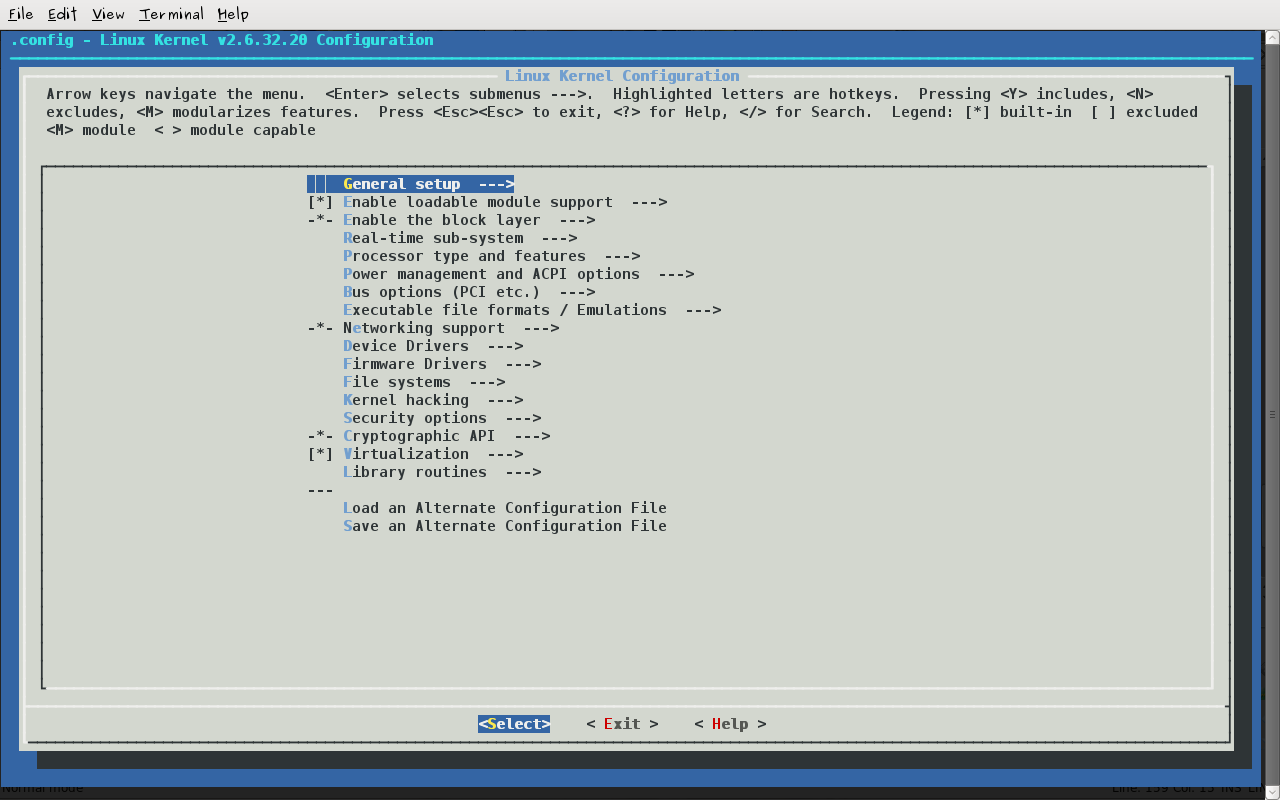
\includegraphics[width=13cm]{images/PrimeiraTela.png}
      \end{figure}

  \subsection{Configurando o \emph{Kernel}}
    \paragraph{}
    Após abrir a tela de configuração do \emph{Kernel} pode-se ver várias opções, vamos fazer uma análise de cada uma e propor 
    alguma configurações para o nosso contexto. Contudo deve ficar claro que as opções são muito flexíveis.

  \newpage
  \subsubsection{General Setup - Configurações gerais}
    \paragraph{}
    Acesse o menu \emph{``General Setup``}, esta contém diversas configurações de proposito geral.
      \begin{figure}[ht]
	\center
	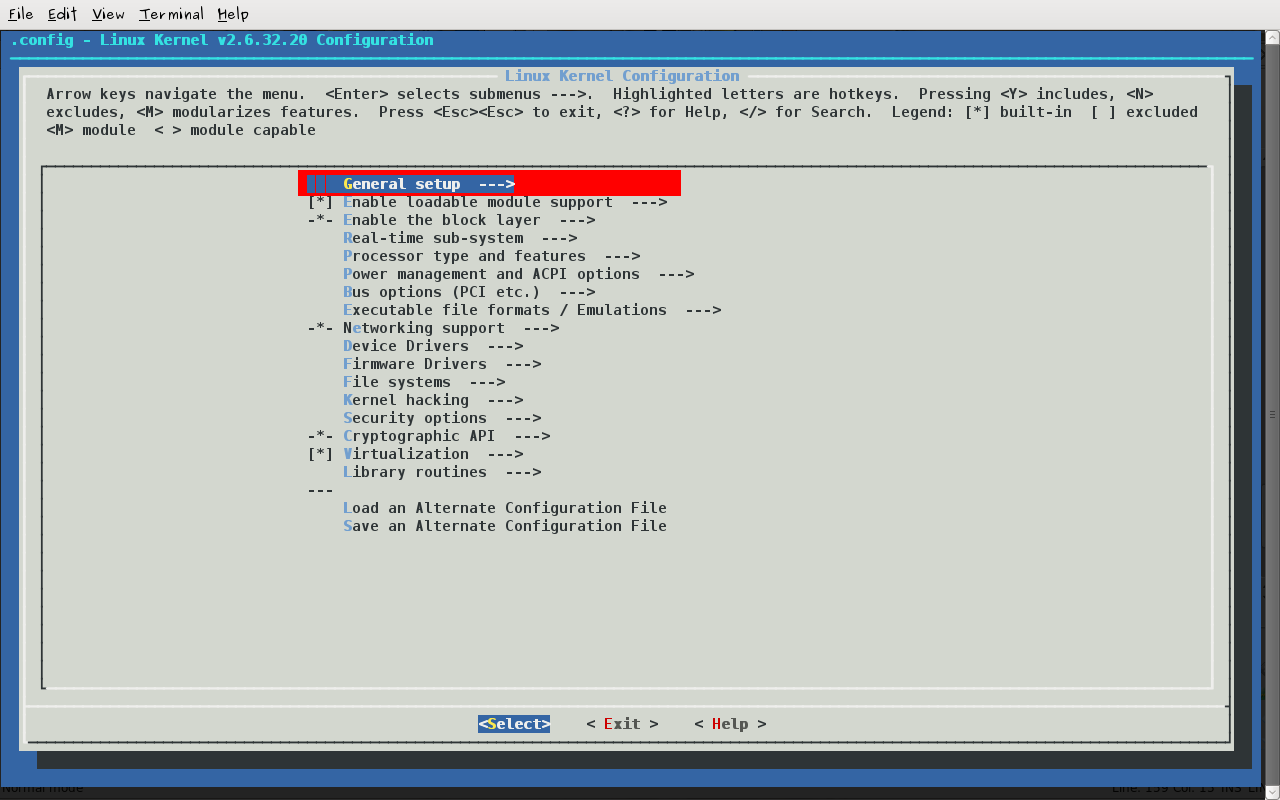
\includegraphics[width=10cm]{images/GeneralSetupInit.png}
      \end{figure}

    \paragraph{}
    Após acessar este menu a tela modifica-se para um submenu, semelhante ao apresentado abaixo:
      \begin{figure}[ht]
	\center
	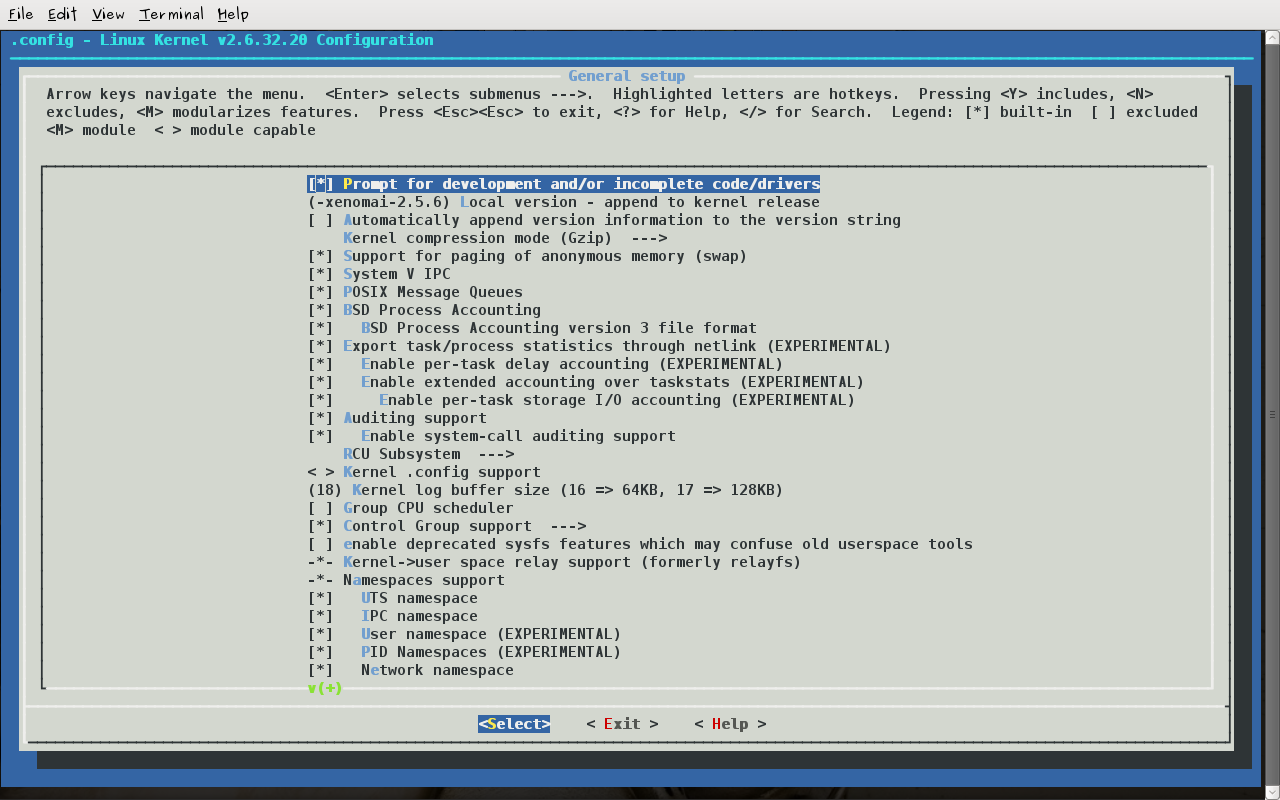
\includegraphics[width=10cm]{images/GeneralSetup1.png}
      \end{figure}

    \newpage
    \paragraph{}
    Segue uma breve descrição sobre as principais opções:
      \begin{itemize}
	\item \textbf{Prompt for development and/or incomplete code/drivers}: Muitos dos suportes fornecidos pelo \emph{Linux} 
	      (\emph{drivers} de rede, sistemas de arquivos, protocolos de rede, etc) podem estar em estado de desenvolvimento, isto 
	      significa que as funcionalidades, a estabilidade, ou o nível de teste ainda não é alto o bastante para uso geral. Este 
	      estado é frequentemente conhecido por versão \emph{''alpha-test``}. Em geral é desencorajado que desenvolvedores utilizem 
	      tais versões para evitar problemas de não funcionamento. \\
	      Contudo esta opção também tornará \emph{drives} obsoletos ativos. Para este tutorial recomenda-se deixa esta opção selecionada.
	\item \textbf{Local version - append to kernel release}: Adiciona uma \emph{string} extra no fim da versão do seu \emph{Kernel}. Para  
	      visualizar o nome do \emph{Kernel}, basta utilizar o comando \emph{uname -r } ou vê-lo na tela inicial do gerenciador de boot. 
	      Se você adicionar caracteres neste campo, compilar e instalar o \emph{Kernel} então você notará por meio do comando \emph{uname}
	      que o os caracteres que você inseriu fazem parte do nome do \emph{Kernel}. O tamanho máximo pode ser de 64 caracteres.\\
	      Nesta opção digite: \emph{-xenomai-2.5.6}
	\item \textbf{Automatically append version information to the version string}: Esta opção tentará determinar automaticamente se a 
	      atual versão da árvore de diretório é uma versão da árvore, procurando pela \emph{tag} GIT\footnote{GIT é um sistema de controle 
	      de versão distribuído com ênfase em velocidade. } que pertencem a atual árvore revisada.\\
	      Uma \emph{string} no formato -gxxxxxxxx será adicionada para o \emph{localversion} se um GIT baseado na árvore for encontrado.
	      A \emph{string} gerada para ele será adicionada depois de qualquer marca \emph{localversion*} em arquivos o valor é ajustado em 
	      CONFIG\_LOCALVERSION.\\
	      Isto é requerido para \emph{Perl}, e um repositório GIT, mas não é necessário que o GIT ou \emph{cogito tools} seja instalado.\\
	      Recomendamos que esta opção seja desmarcada para o nosso contexto.
	\item \textbf{Kernel compression mode (Gzip)}: Esta opção lida com os possíveis algoritmos responsáveis pela compressão do \emph{Kernel}. 
	      As seguintes opções estão disponíveis:
	      \begin{itemize}
	      \item \textbf{Gzip}:Dentre os algoritmos é aquele que possui a menor taxa de compressão, contudo é o mais rápido de todos.
	      \item \textbf{Bzip2}: Possui uma taxa de compressão e velocidade intermediárias. A velocidade de descompressão é a mais lenta entre
		      as opções. O tamanho do \emph{Kernel} é cerca de 10\% menor que o \emph{gzip}. Além disto utiliza uma quantidade de memória
		      maior.
	      \item \textbf{LZMA}:O mais recente algoritmo de compressão. A taxa de compressão é a melhor, a velocidade de descompressão esta 
		      entre as duas opções e a compressão é a mais lenta. O tamanho do \emph{kernel} chega a ficar 33\% menor com LZMA em
		      comparação com \emph{gzip}.
	      \end{itemize}
	      Para o nosso contexto mantenha a opção \emph{gzip} seleciona.
	\item \textbf{Support for paging of anonymous memory (swap)}: Esta opção permite que vocês escolha se deseja ter suporte para escalonar 
		os chamados dispositivos de \emph{swap} ou arquivos \emph{swap} no seu \emph{Kernel}. Eles são utilizado para aperfeiçoar a memória 
		virtual melhorando o trabalho com a sua memória RAM.\\
		Para o nosso contexto mantenha esta opção selecionada.
	\item \textbf{System V IPC}: Comunicação inter processo é um conjunto de bibliotecas e chamadas de sistemas que deixa os processos 
		sincronizado e permite a troca de informações entre eles.\\
		Mantenha esta opção selecionada.
	\item \textbf{POSIX Message Queues}: É uma variante da fila de mensagem que é parte do IPC.\\ 
		Recomenda-se manter esta opção selecionada.
	\item \textbf{BSD Process Accounting}: Um programa com nível de usuário será capaz de instruir o \emph{kernel} (através de uma chamada 
		especial do sistema) para gravar informações sobre o processos em um arquivo: sempre que um processo termina, as informações 
		sobre esse processo são adicionadas pelo \emph{Kernel} ao final do arquivo. A informação inclui coisas como o tempo de criação, 
		usuário proprietário, nome do comando, uso de memória, controle de terminal etc. Recomenda-se manter esta opção selecionada.
	\item \textbf{Auditing support}: Habilita infraestrutura de auditoria que pode ser utilizada dar suporte para outros subsistemas do 
		\emph{kernel}, assim como \emph{SELinux}\footnote{provê uma política de segurança sobre todos os processos e objetos do sistema 
		baseando suas decisões em etiquetas contendo uma variedade de informações relevantes à segurança.}. \\
		Recomenda-se deixar esta opção marcada.
	\item \textbf{Enable system-call auditing support}: Habilita uma baixa sobrecarga de chamadas do sistema.
	\item \textbf{RCU Subsystem}: emph{Read-copy-update} (RCU) é um mecanismo de sincronização implementando um tipo de exclusão mutua que 
	      pode ser usado as vezes como uma alternativa para trancas \emph{readers-writer}. Contudo, atualizações RCU podem ser caras.
	\item \textbf{Group CPU scheduler}: Esta características deixa o escalonador da CPU reconhecer grupos de tarefas e controlar a largura 
		de banda alocada para conjunto de tarefas de grupos. 
	\item \textbf{Kernel .config support}: Esta opção habilita o completamente o arquivo do \emph{Kernel} do Linux '.config' para ser salvo 
	      no \emph{Kernel}. 
	\item \textbf{Configure standard kernel features (for small systems)}: Esta opção permite que certas bases da opção do \emph{kernel} e 
		configurações sejam desabilitada. Isto é para ambiente especiais que podem ser tolerante a um \emph{kernel} 'não-padrão'. Somente 
		utilize esta opção se você realmente sabe o que esta fazendo.
    \end{itemize}

%---------------------------------------------------------------------------------------------------------------------------
%--------------------------------- SEÇÃO: LKM ------------------------------------------------------------------------------
%---------------------------------------------------------------------------------------------------------------------------
  \subsubsection{Enable loadable module support}
    \paragraph{}
    Um módulo de \emph{kernel} é um arquivo objeto que contém códigos para estender a execução do \emph{kernel}, ou então chamar a
    base do \emph{kernel} de um sistema operacional. São tipicamente utilizados para adicionar suporte para hardware e/ou sistemas de 
    arquivo, ou para chamadas de sistemas.
      \begin{figure}[ht]
	\center
	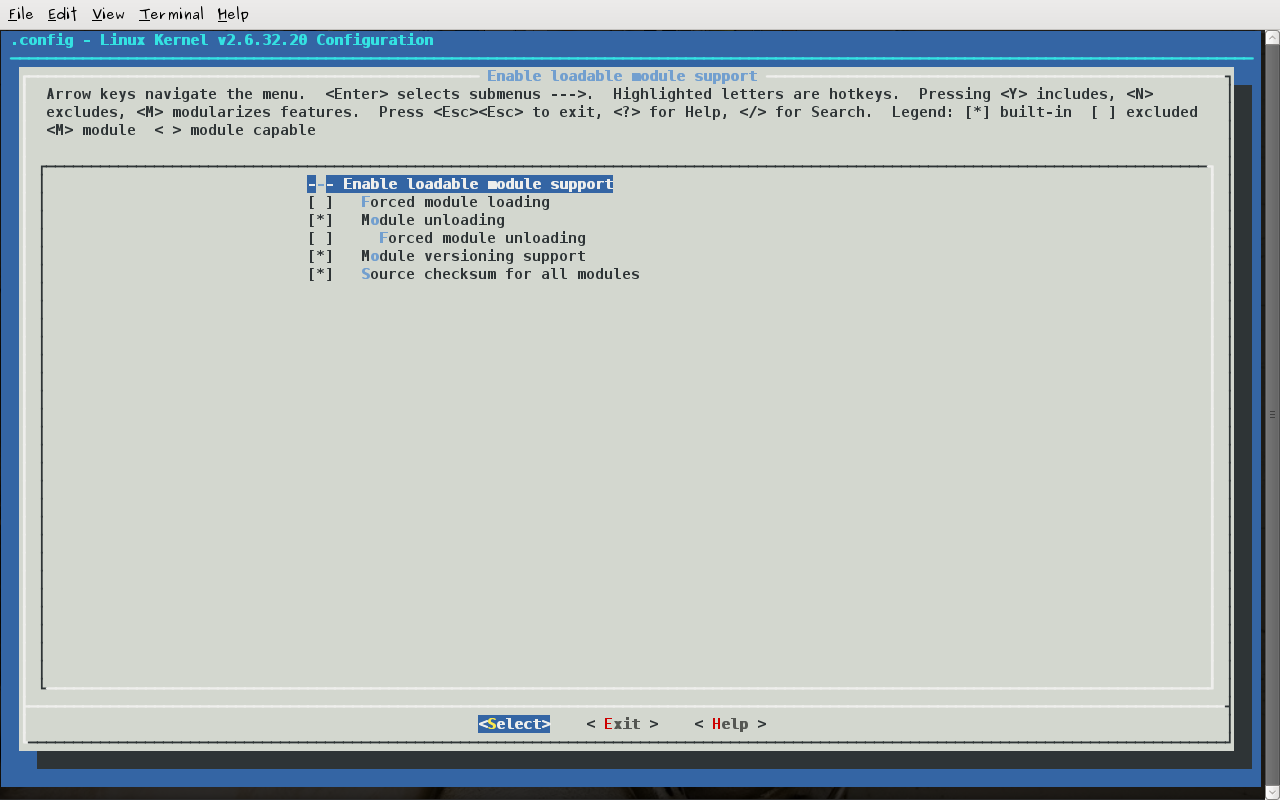
\includegraphics[width=10cm]{images/EnableLoadableModuleSupport.png}
      \end{figure}

    \paragraph{}
    Segue uma breve descrição sobre as principais opções:
      \begin{itemize}
      \item \textbf{Enable loadable module support}: Módulos do \emph{Kernel} são pequenos pedaços de código compilado que podem ser 
	  inseridos em um \emph{kernel} executando, ou então iniciar permanentemente dentro de um \emph{Kernel}. Utiliza-se a ferramenta 
	\emph{modprobe} para adicionar (e as vezes remover) os módulos. Se você marcar esta opção, muitas partes do \emph{Kernel} podem 
	  ser construída como módulos (responde M em vez de Y onde é indicado): isto é mais útil para opções não muito frequentes que não 
	  são requeridas durante o \emph{boot}.\\
	  Se você disser Y aqui, você precisará rodar \emph{make modules\_install} para inserir módulos sobre /lib/modules onde \emph{modprobe}
	  pode encontra-lo (você pode precisar ser root para fazer isto).
      \item \textbf{Module unloading}: Sem esta opção você não será capaz de descarregar qualquer modulo (note que alguns módulos podem não 
	  ser descarregáveis de qualquer forma), que faz seu \emph{Kernel} levemente menor e simples.
      \item \textbf{Forced module unloading}: Esta opção permite você forçar um modulo para ser carregado, mesmo se o \emph{Kernel} acreditar 
	  que seja inseguro: o \emph{Kernel} irá remover o modulo sem esperar que qualquer um para de usa-lo. 
      \item \textbf{Source checksum for all modules}: Modulo que contém um MODULE\_VERSION pegam um campo extra \emph{srcversion} dentro da sua 
	  seção \emph{modinfo}, que contenha uma soma dos arquivos fontes para fazer o \emph{checksum}.
      \end{itemize}

%---------------------------------------------------------------------------------------------------------------------------
%--------------------------------- SEÇÃO: ENABLE THE BLOCK LAYER -----------------------------------------------------------
%---------------------------------------------------------------------------------------------------------------------------
  \subsubsection{Enable the block layer}
    \paragraph{}
    Permite que a camada de bloco possa ser removida de um \emph{Kernel} se esta não for necessária (sobre algum dispositivo embarcado
    por exemplo). Se esta opção é desabilitada, então os arquivos \emph{blockdev} tornam-se inutilizáveis e algum sistema de arquivos
    (assim como \emph{ext3}) tornará-se indisponível. Esta opção também desabilitará característica do SCSI e armazenamento USB.

%---------------------------------------------------------------------------------------------------------------------------
%--------------------------------- SEÇÃO: PROCESSO TYPE AND FEATURE --------------------------------------------------------
%---------------------------------------------------------------------------------------------------------------------------
  \subsubsection{Processor type and features}
    \paragraph{}
    Se você deseja ter um \emph{Kernel} do Linux executando o mais rápido possível para o seu processador especifico e tipo de hardware, 
    neste submenu você poderá ajusta-lo para pegar até o último bit de performasse de saída do seu hardware. 

    \begin{figure}[ht]
    \center
    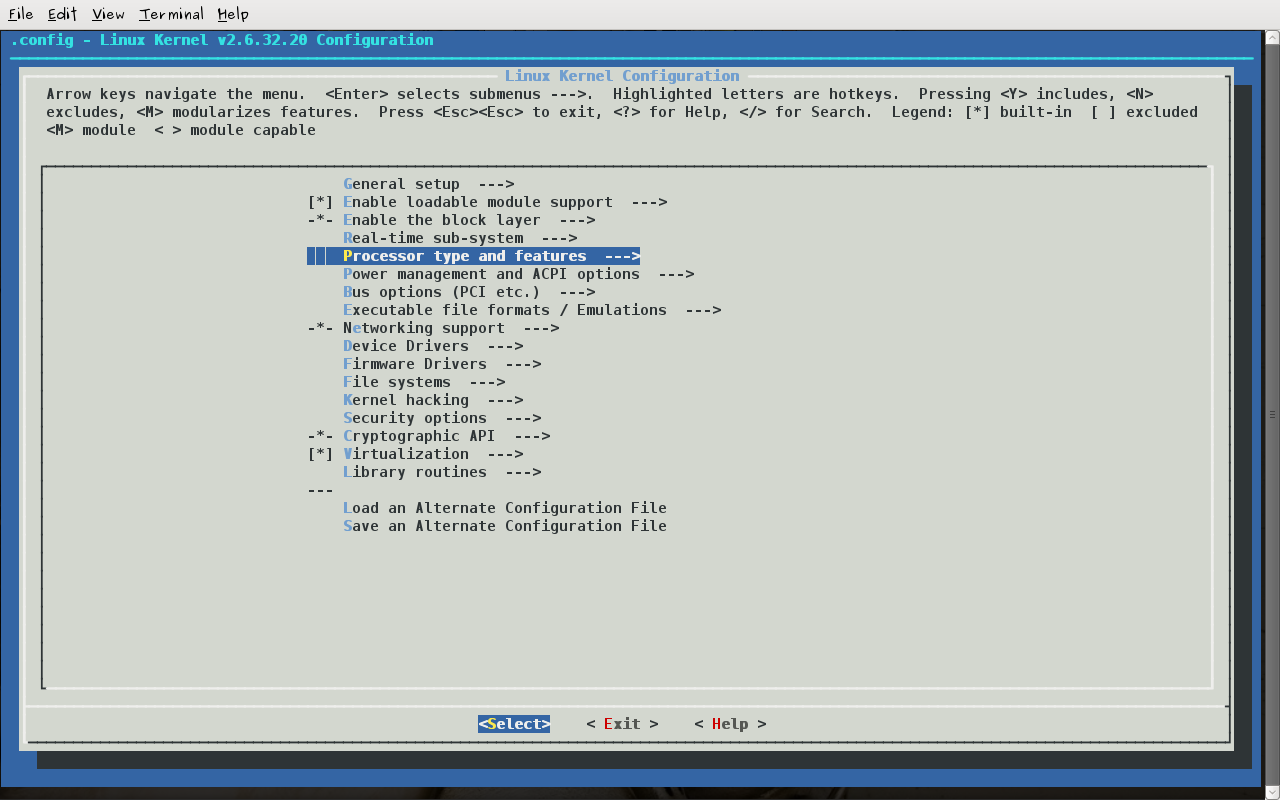
\includegraphics[width=10cm]{images/ProcessoTypeAndFeature.png}
    \end{figure}

  \paragraph{}
    Segue uma breve descrição sobre as principais opções:
    \begin{itemize}
    \item \textbf{Tickless System (Dynamic Ticks)}: A menos que você precise da menor latência\footnote{ é a diferença de tempo entre o 
	    início de um evento e o momento em que seus efeitos tornam-se perceptíveis} possível, utilize \emph{Dynamic ticks} para assegurar 
	    que interrupções do \emph{timer} serão disparadas quando necessárias.
    \item \textbf{High Resolution Timer Support}: A maioria dos sistema relativamente modernos (Pentium 3 e superiores) tem um \emph{timer} de 
	    alta resolução, aceitando tempos mais precisos. Não é realmente obrigatório, mas algumas aplicações com \emph{mplayer} podem 
	    beneficiar-se da utilização.\\
	    Contudo para este documento, mantenha esta opção desmarcada.
    \item \textbf{Symmetric multi-processing support}: Se você tem habilitado múltiplas CPUs (idênticas) ou sua CPU tem múltiplos núcleos, 
	    habilite esta opção.
    \item \textbf{Single-depth WCHAN output}: WCHAN é a abreviação para \emph{waiting channel} (esperando por canal) e identifica onde tarefas 
	    estão atualmente esperando. Com esta opção habilitada, o calculo para a espera do canal é simplificada por conta da precisão. Muitos 
	    usuários não precisão deste nível de precisão e a simplificação significa menos sobrecarga do escalonador.
    \item \textbf{Processor family(Processor ...)}: Você deve selecionar a família de processador da sua CPU.
    \item \textbf(SMT (Hyperthreading) scheduler support): Esta deve ser selecionada se você tem um chip Pentium com suporte para 
	    \emph{hyperthreading}. Esta opção não é obrigatória (o \emph{Kernel} irá rodar bem sem ele) mas deve aperfeiçoar as decisões tomadas 
	    pelo escalonador do \emph{kernel}.
    \item \textbf{HPET Timer Support}: Suporte para \emph{High Precision Event Timer}, que pode ser visto como um recurso de 
	    fonte de tempo sobre algo mais moderno. Especialmente se você tem mais de um núcleo/CPU, permitindo que este ofereça acesso 
	    ''mais barato`` do que sem o apoio do HPET.
    \item \textbf{Multi-core scheduler support}: Habilite esta opção se você tiver uma CPU com múltiplos núcleos internamente; isto irá melhorar 
	    a performasse do escalonador.
    \item \textbf{Preemption Model (Preemptible Kernel (Low-Latency Desktop))}: O \emph{kernel} permite diferentes modelos de preempção para 
	    trabalhar com uma grande variedade de situações. Preempção é a habilidade de um \emph{kernel} interromper a si mesmo enquanto ele 
	    estiver fazendo outra coisa, para trabalhar com algo com a prioridade maior. 
	    \begin{itemize}
	      \item No Forced Preemption - Forçar preempção.
	      \item Voluntary Kernel Preemption - onde um processo com baixa prioridade pode voluntariamente ceder tempo de CPU.
	      \item Preemptible Kernel (Low-Latency Desktop)- onde todo processo pode ceder tempo de CPU (assim como eles não podem entrar em uma 
	      região crítica no momento)
	    \end{itemize}
	    Escolha a última opção para este documento.
    \item \textbf{Machine Check / overheating reporting}: MC permite ao processo notificar o \emph{kernel} quando problemas são detectados (assim 
	    como sobrecarga); baseado-se na sua severidade, o \emph{Kernel} do Linux pode reportar o assunto ou tomar uma ação imediata.
    \item \textbf{Memory Model (Sparse Memory)}: Se você tem um processador de 32 bits, selecione a memória \emph{Flat} que você precisa. CPUs 
	    com espaço de endereçamento grande (assim como CPUs de 64 bits) provavelmente só permitem que você selecione \emph{Sparse Memory}. 
	    Quando \emph{Sparse Memory} é selecionado \emph{Sparse Memory virtual memmap} deve ser selecionado também.
    \item \textbf{MTRR (Memory Type Range Register) support}: Com suporte para MTRR, aplicações como o servidor X podem ser controladas como o 
	    processador armazena os acessos à memória, aumentando a performasse para leitura/escrita para cetas faixas de memória.
    \item \textbf{Enable -fstack-protector buffer overflow detection}: Esta opção torna ligado a característica -fstack-protector GCC. Esta 
	    característica insere, no inicio das funções, um \emph{canary value} \footnote{é um estrategia para detectar ataques de transbordo 
	    em tempo de execução, sem requerer que o programador mude o seu código} sobre a pilha um pouco antes do endereço de retorno e
	    valida o valor antes de realmente voltar. Pilhas que transportam do seu tamanho agora também sobrescrevem o \emph{canary}, que quando 
	    é detectado e quando o ataque é neutralizado via \emph{kenel panic}. Esta característica só esta disponível para versões do gcc 4.2 
	    ou superior.
	  \\Para este documento desmarque esta opção.
    \end{itemize}

%---------------------------------------------------------------------------------------------------------------------------
%--------------------------------- SEÇÃO: POWER MANAGEMENT AND ACPI OPTION -------------------------------------------------
%---------------------------------------------------------------------------------------------------------------------------
  \subsubsection{Power Management And ACPI options}
  \paragraph{}
  O gerenciado de energia fornece opções de economia de energia para característica do Linux, não somente para 
  APM\footnote{Advanced Power Management: uma norma de gerenciamento de energia usada inicialmente em computadores portáteis}/ACPI
  \footnote{Advanced Configuration and Power Interface: usado para configuração e gerenciamento de energia do computador.}, 
  mas também para supender RAM e modo de descanço.
  \begin{figure}[ht]
  \center
  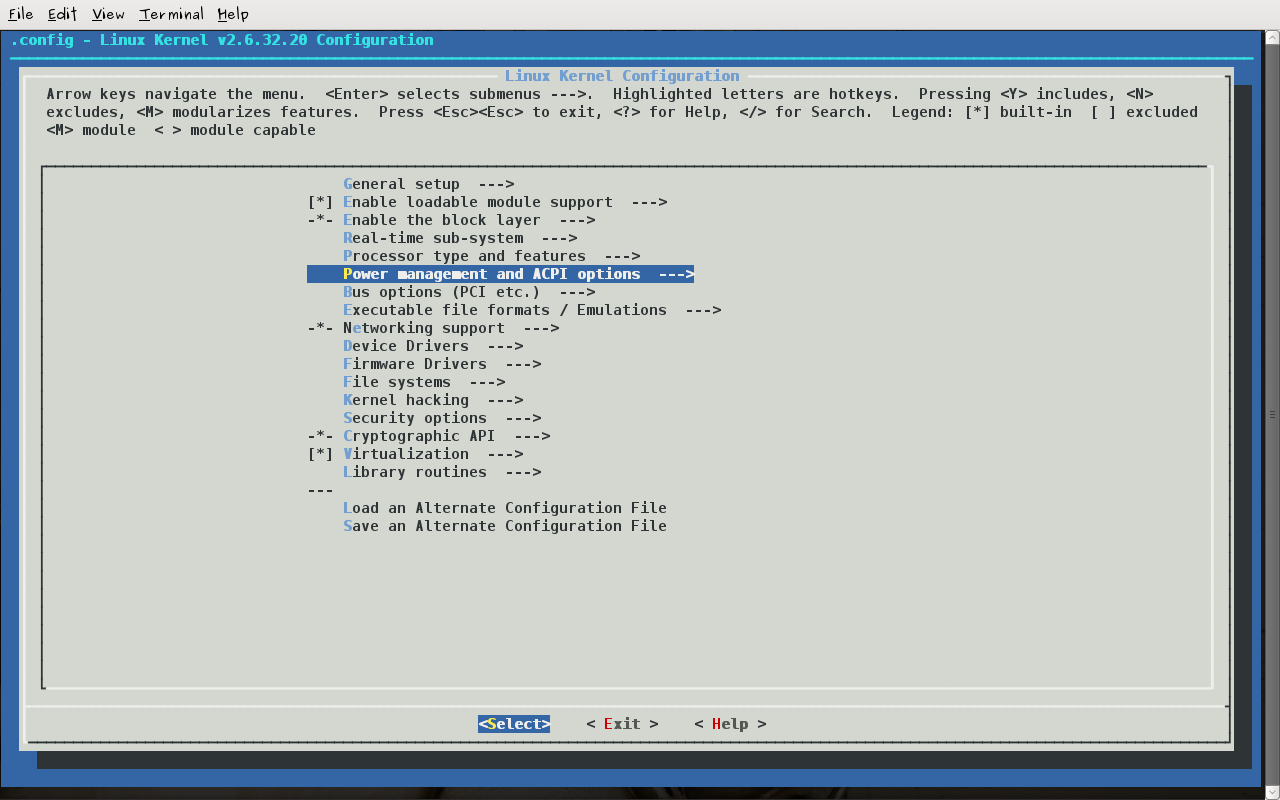
\includegraphics[width=10cm]{images/PowerManagementAndACPIoptions.png}
  \end{figure}
  \paragraph{}
  Segue uma breve descrição sobre as principais opções:
  \begin{itemize}
  \item \textbf{Power Management Support}
	\\Habilita esta opção permite selecionar uma ou mais opções de gerenciamento de energia.
  \item \textbf{Suspend to RAM and standby}
	\\Se você tiver momentos em que temporariamente você deixe o seu sistema mas não deseja desliga-lo e inicializa-lo novamente
	  depois, você pode optar por ter o sistema suspendendo por conta própria dentro da memória - neste caso, muito dispositivos
	  que consumem muita energia serão desligado mas você não perderá nenhuma informação assim tudo fica mantido na memória (e a
	  memória mantém-se ligada).
  \item \textbf{Hibernation (aka 'suspend to disk')}
	\\Em hibernar, todo dispositivo desliga. O estado atual do sistema (tal como conteúdo da memória) é salvo dentro do espaço de swap.
	  Quando você da boot no seu sistema, o Kernel do Linux irá detectar que o espaço de swap e carregará toda a informação de volta
	  para dentro da memória.
  \item \textbf{ACPI (Advanced Configuration and Power Interface) Support}
	\\Nesta seção você pode configurar vários aspectos de suporte ACPI. Habilitando APCI pode ser de grande ajuda para reduzir o 
	  consumo de energia. Infelizmente, nem todo dispositivo segue a especificação ACPI a risca. Você terá que encontrar tópicos
	  na internet onde falhas de boot ou irregularidade de rede podem ser resolvidas desabilitando uma parte do suporte ACPI.
	\\Para este documento recomendamos desmarcar a opção ''processor``, ''APM(Advanced Power Management) BIOS Support``
  \item \textbf{CPU Frequency Scaling}
	\\Se você tem um laptop você irá querer habilitar ''CPU Frequency scaling`` para reduzir a velocidade da CPU (e o consumo de energia
	  com isto) quando a CPU não estiver sendo utilizada.
	\\Para o contexto deste documento desmarque esta opção
  \end{itemize}

%---------------------------------------------------------------------------------------------------------------------------
%--------------------------------- SEÇÃO: DEVICE DRIVE ---------------------------------------------------------------------
%---------------------------------------------------------------------------------------------------------------------------
  \subsubsection{Device Drivers}
  \paragraph{}
  Nesta seção você pode configurar suporte para vários tipos de dispositivo no seu sistema. É com esta configuração que é necessária para 
  o comando lspci (e outras informações do sistema) mostrar as suas saídas. Esta é uma opção do seu sistema muito especifica, por isto não
  é possível propor uma configuração geral. Contudo para o contexto deste documento acesse: Input device support --->, Miscellaneous device --->,
  PC Speaker support e Desabilitar esta opção.

%---------------------------------------------------------------------------------------------------------------------------
%--------------------------------- SEÇÃO: COMPILANDO O KERNEL --------------------------------------------------------------
%---------------------------------------------------------------------------------------------------------------------------
  \section{Compilando o Kernel}
  \paragraph{}
  Para compilar o Kernel execute o comando abaixo no diretório /usr/src/linux: 
	{\small  
  \begin{verbatim}CONCURRENCY_LEVEL=2 CLEAN_SOURCE=no fakeroot make-kpkg --initrd kernel_image kernel_headers
  \end{verbatim}
	} 

%---------------------------------------------------------------------------------------------------------------------------
%--------------------------------- SEÇÃO: INSTALAÇÃO DO NOVO KERNEL --------------------------------------------------------
%---------------------------------------------------------------------------------------------------------------------------
\section{Instalando o novo Kernel}
  \paragraph{}
  No diretório /usr/src digite:
	{\small  \begin{verbatim}dpkg -i linux-image*.deb\end{verbatim}     }


%---------------------------------------------------------------------------------------------------------------------------
%--------------------------------- SEÇÃO: INITRD E BOOT --------------------------------------------------------------------
%---------------------------------------------------------------------------------------------------------------------------
\section{Construindo initrd e atualizando o gerenciador de boot}
  \paragraph{}
  Construindo o initrd e atualizando o gerenciador de boot
	{\small  \begin{verbatim}update-initramfs -c -k 2.6.32.20-xenomai-2.5.6 && update-grub\end{verbatim}     } 


%---------------------------------------------------------------------------------------------------------------------------
%--------------------------------- SEÇÃO: BIBLIOGRAFIA ---------------------------------------------------------------------
%---------------------------------------------------------------------------------------------------------------------------
%\newpage
%\section{Bibliografia}
%\begin{enumerate}
% \item http://packages.debian.org/squeeze/kernel-package
% \item http://packages.ubuntu.com/lucid/libncurses5-dev
% \item http://packages.debian.org/squeeze/zlib1g-dev
% \item www.gnu.org/software/ncurses/ncurses.html
% \item The MINIX 3 Operating System
% \item Towards Real Microkernels,  Liedtke, Jochen
% \item http://www.xenomai.org/documentation/xenomai-2.5/README.INSTALL
% \item http://www.xenomai.org/index.php/Building\_Debian\_packages 
% \item http://cateee.net/lkddb/web-lkddb/EXPERIMENTAL.html
% \item http://how-to.wikia.com/wiki/How_to_configure_the_Linux_kernel
% \item http://swift.siphos.be/linux_sea/ch07.html
%\end{enumerate}


\end{document}